\chapter{SSH (Secure Shell)}\label{ssh-secure-shell}

\section{Console Port Security}\label{console-port-security}

\begin{itemize}
\tightlist
\item
  By DEFAULT, no password us needed to access the CLI of a CISCO IOS
  DEVICE via the CONSOLE PORT
\item
  You can CONFIGURE a PASSWORD on the \emph{console line}

  \begin{itemize}
  \tightlist
  \item
    A USER will have to enter a PASSWORD to ACCESS the CLI via the
    CONSOLE PORT
  \end{itemize}
\end{itemize}

\begin{figure}
\centering
\pandocbounded{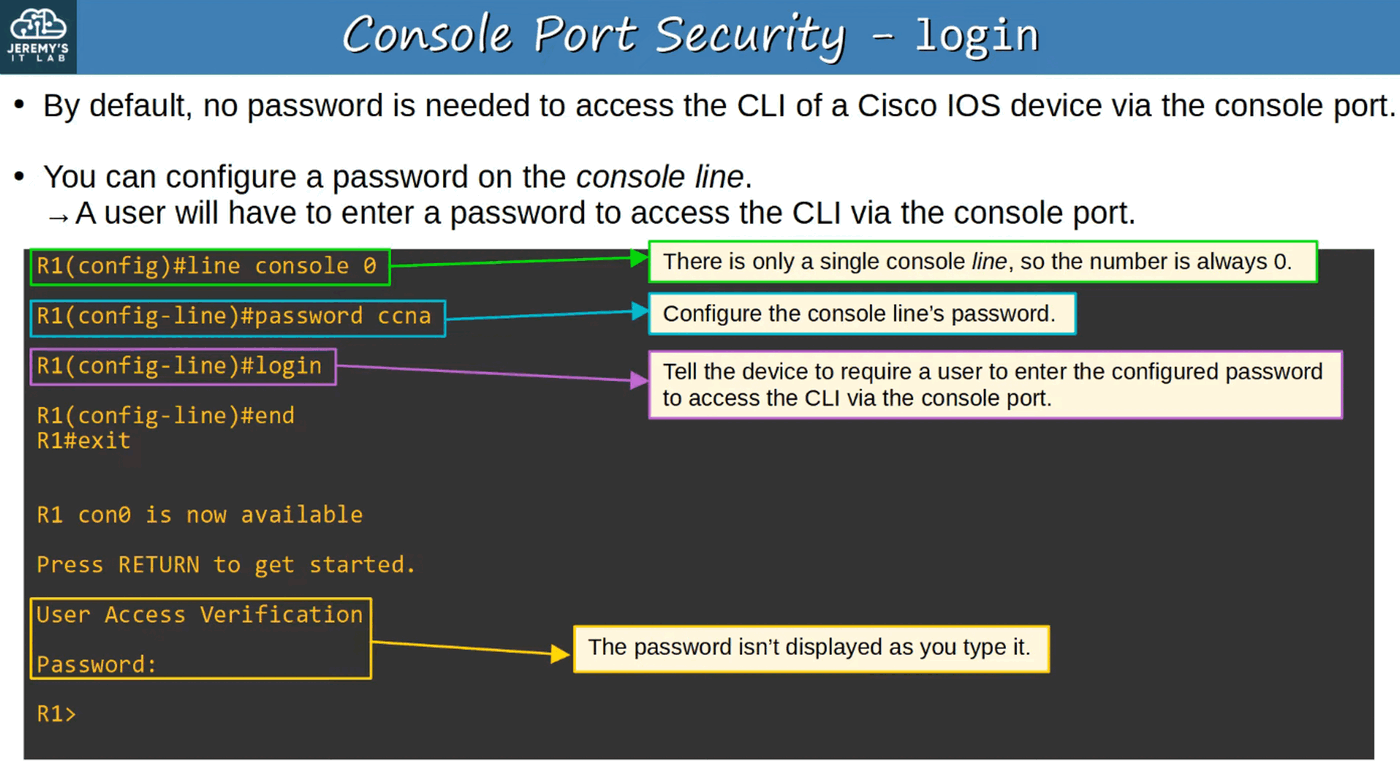
\includegraphics[keepaspectratio,alt={image}]{images/43-ssh/img-001.png}}
\end{figure}

\begin{itemize}
\tightlist
\item
  Alternatively, you can configure the CONSOLE LINE to require USERS to
  LOGIN using one of the configured USERNAMES on the DEVICE
\end{itemize}

\begin{figure}
\centering
\pandocbounded{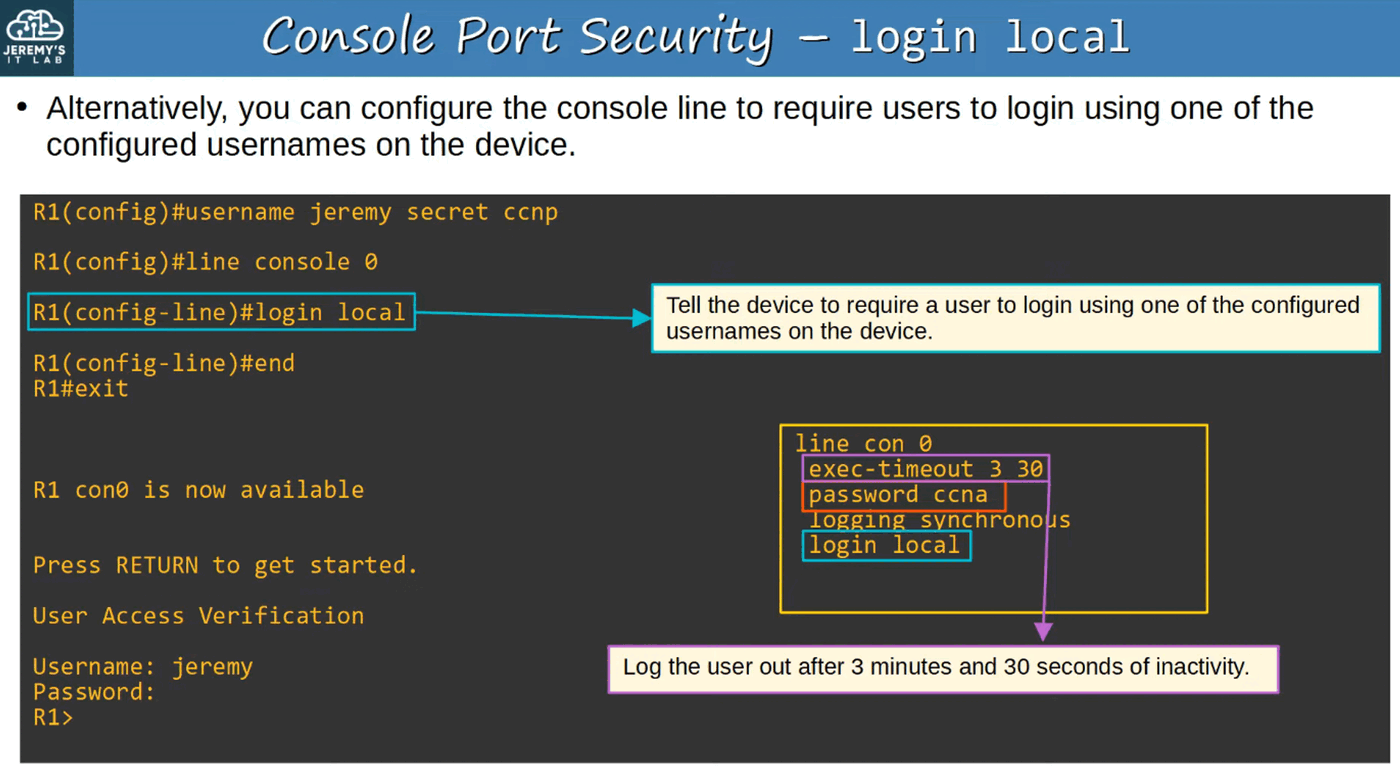
\includegraphics[keepaspectratio,alt={image}]{images/43-ssh/img-002.png}}
\end{figure}

\section{Layer 2 Switch Management
IP}\label{layer-2-switch-management-ip}

\begin{itemize}
\tightlist
\item
  LAYER 2 SWITCHES do not perform PACKET ROUTING and build a ROUTING
  TABLE. They are NOT IP ROUTING aware
\item
  However, you CAN assign an IP ADDRESS to an SVI to allow REMOTE
  CONNECTIONS to the CLI of the SWITCH (using Telnet or SSH)
\end{itemize}

\begin{figure}
\centering
\pandocbounded{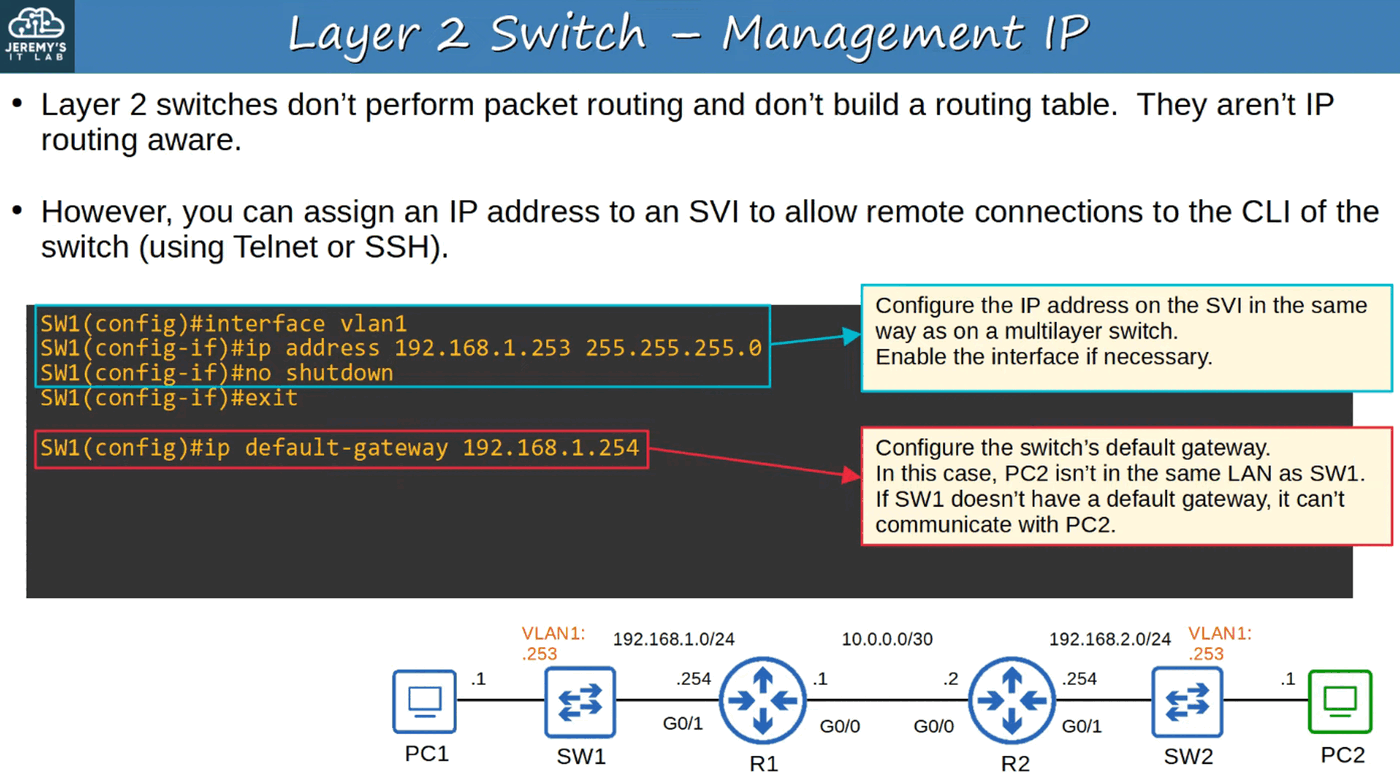
\includegraphics[keepaspectratio,alt={image}]{images/43-ssh/img-003.png}}
\end{figure}

\section{Telnet}\label{telnet}

\begin{itemize}
\tightlist
\item
  TELNET (Teletype Network) is a PROTOCOL used to REMOTELY ACCESS the
  CLI of a REMOTE HOST
\item
  TELNET was developed in 1969
\item
  TELNET has been largely REPLACE by SSH, which is MORE Secure
\item
  TELNET sends data in PLAIN TEXT. NO ENCRYPTION(!)
\end{itemize}

\begin{tipbox}

TELNET SERVERS listen for TELNET traffic on TCP PORT 23

\end{tipbox}

\begin{figure}
\centering
\pandocbounded{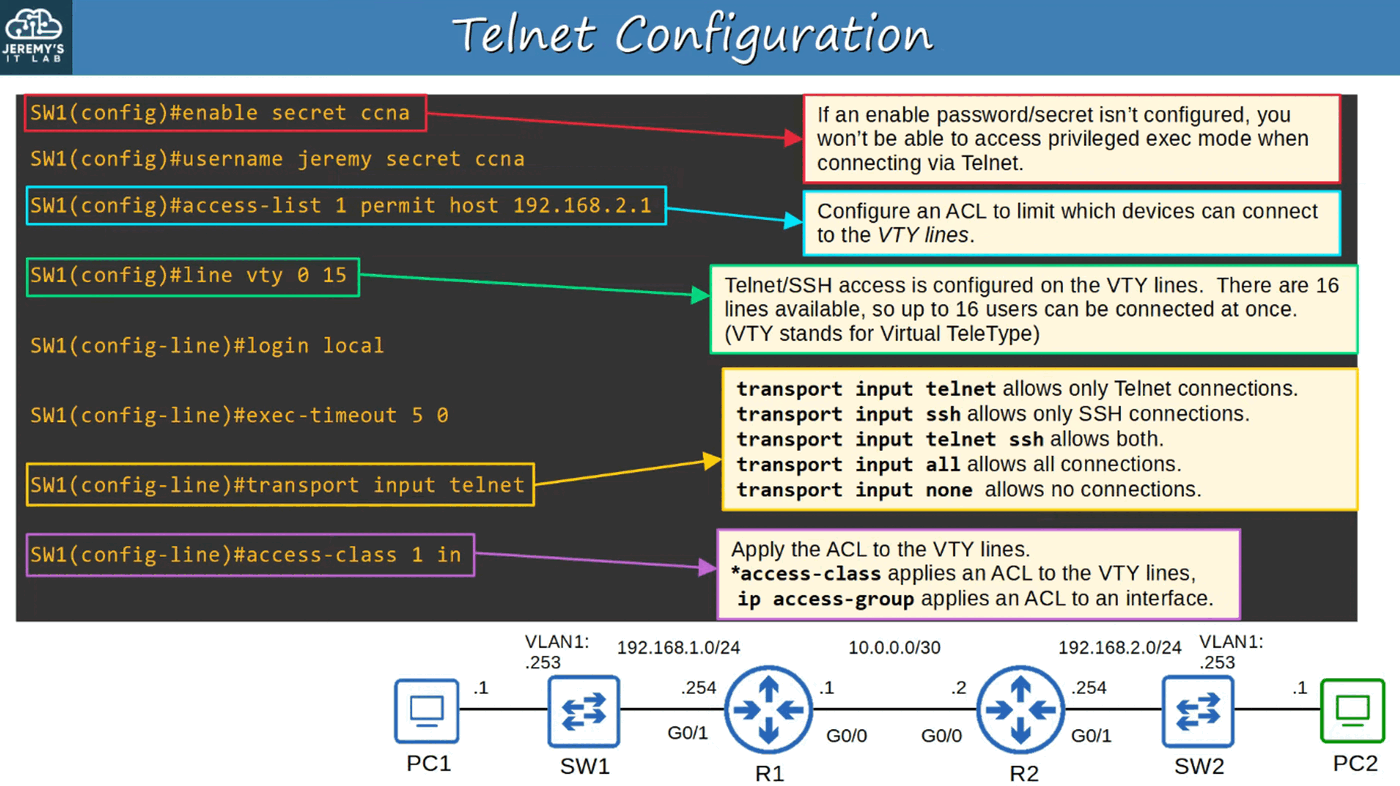
\includegraphics[keepaspectratio,alt={image}]{images/43-ssh/img-004.png}}
\end{figure}

\section{Verify Telnet Configuration}\label{verify-telnet-configuration}

\begin{figure}
\centering
\pandocbounded{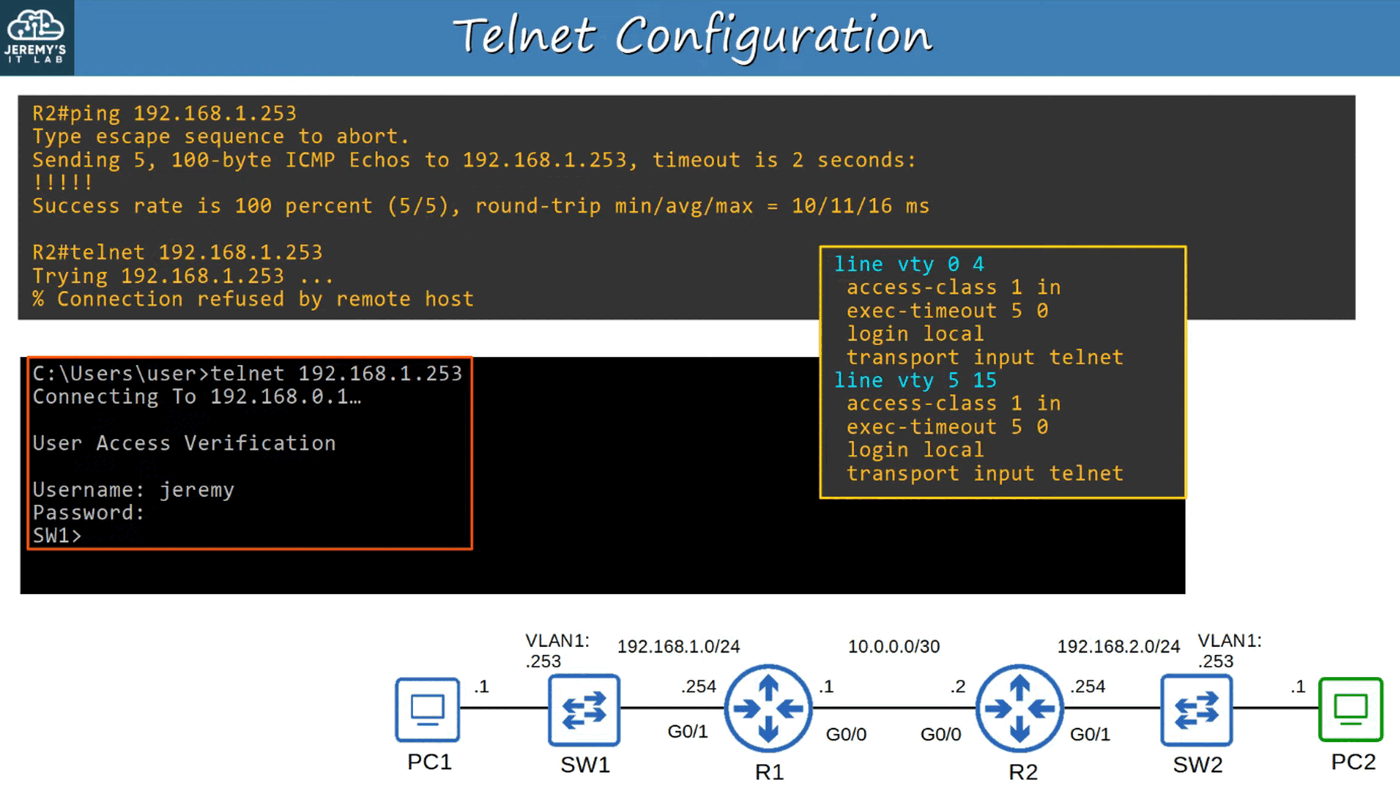
\includegraphics[keepaspectratio,alt={image}]{images/43-ssh/img-005.png}}
\end{figure}

\section{SSH}\label{ssh}

\begin{itemize}
\tightlist
\item
  SSH (Secure Shell) was developed in 1995 to REPLACE LESS SECURE
  PROTOCOLS, like TELNET
\item
  SSHv2, a major revision of SSHv1, was released in 2006
\item
  If a DEVICE supports both v1 and v2, it is said to run `version 1.99'
\item
  Provides SECURITY features; such as DATA ENCRYPTION and AUTHENTICATION
\end{itemize}

\section{Check SSH Support}\label{check-ssh-support}

\begin{figure}
\centering
\pandocbounded{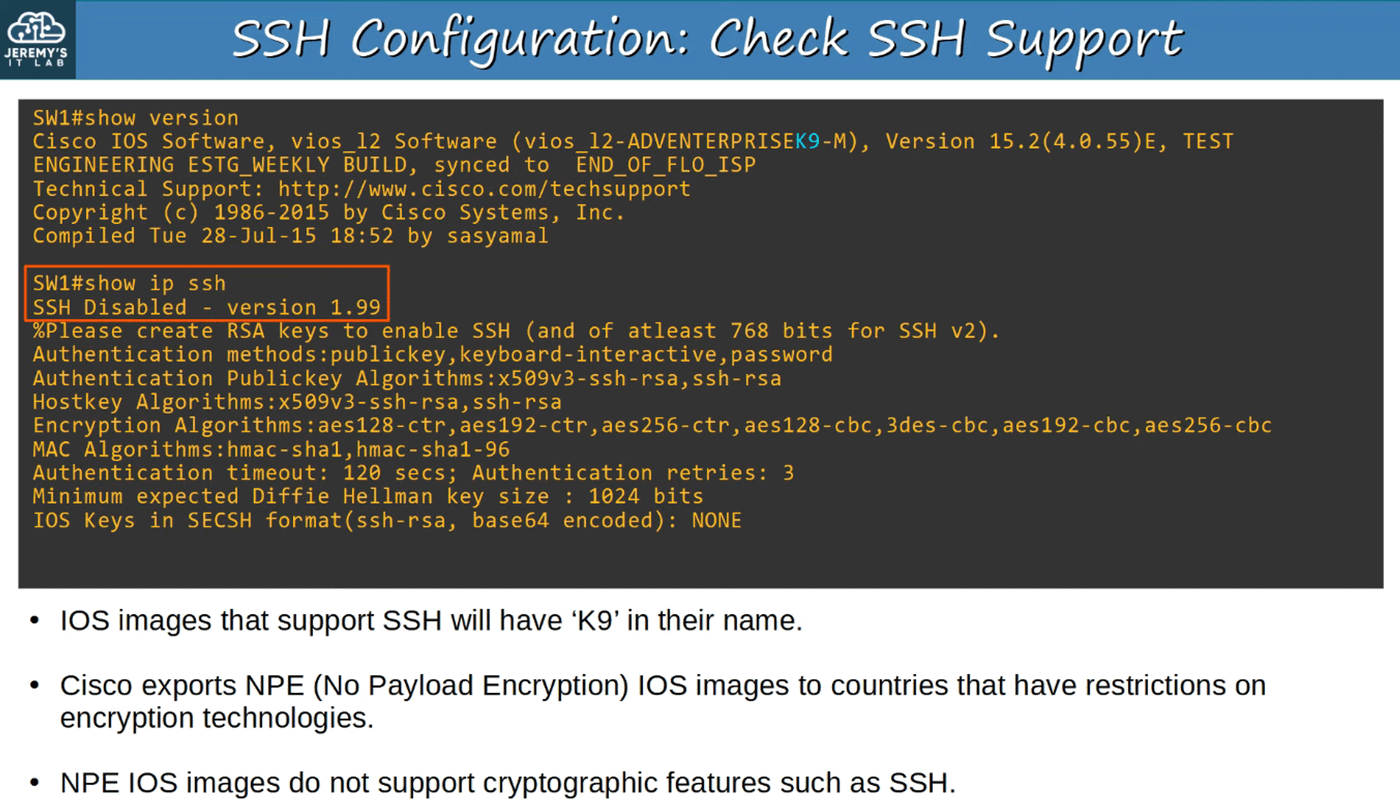
\includegraphics[keepaspectratio,alt={image}]{images/43-ssh/img-006.png}}
\end{figure}

\section{RSA Keys}\label{rsa-keys}

\begin{itemize}
\tightlist
\item
  To ENABLE and use SSH, you must first generate an RSA PUBLIC and
  PRIVATE KEY PAIR
\item
  The KEYS are used for DATA ENCRYPTION / DECRYPTION, AUTHENTICATION,
  etc.
\end{itemize}

\begin{figure}
\centering
\pandocbounded{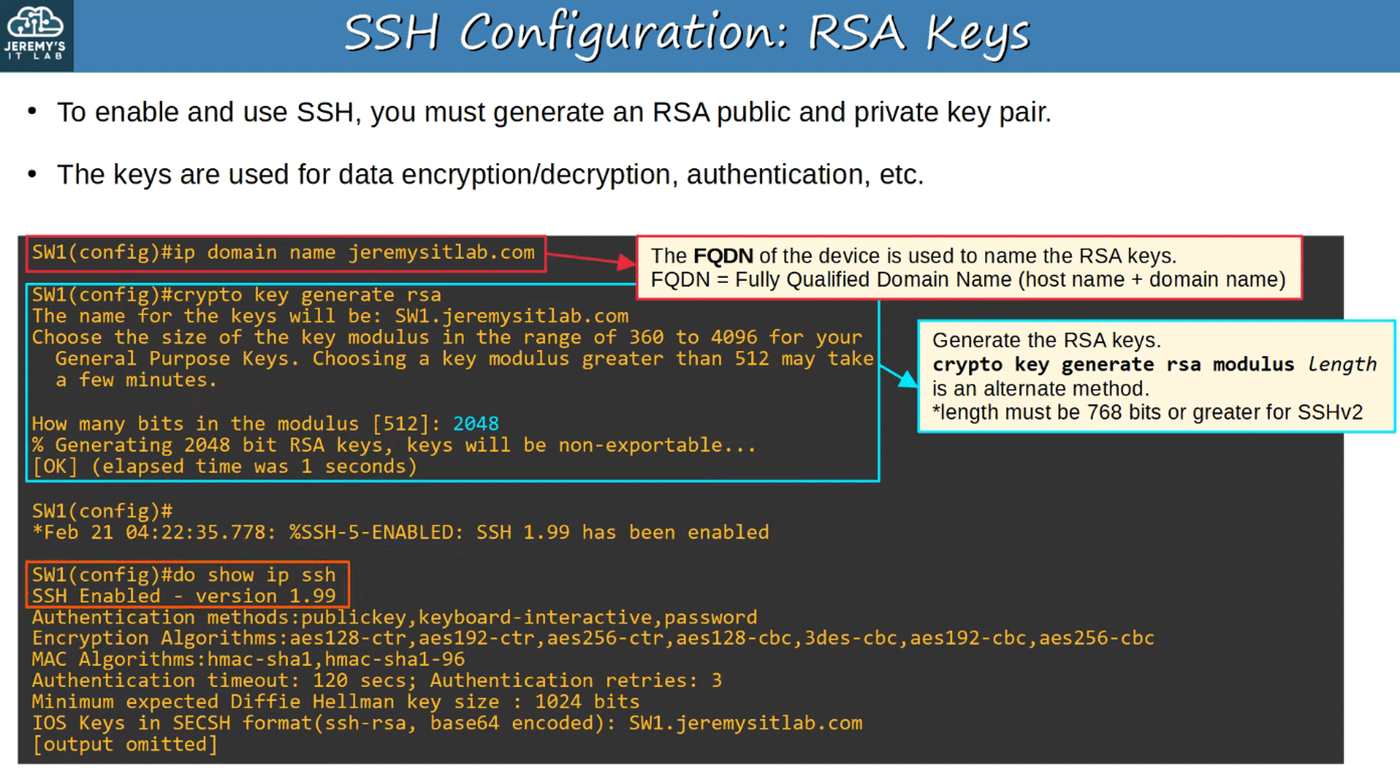
\includegraphics[keepaspectratio,alt={image}]{images/43-ssh/img-007.png}}
\end{figure}

\section{VTY Lines}\label{vty-lines}

\begin{figure}
\centering
\pandocbounded{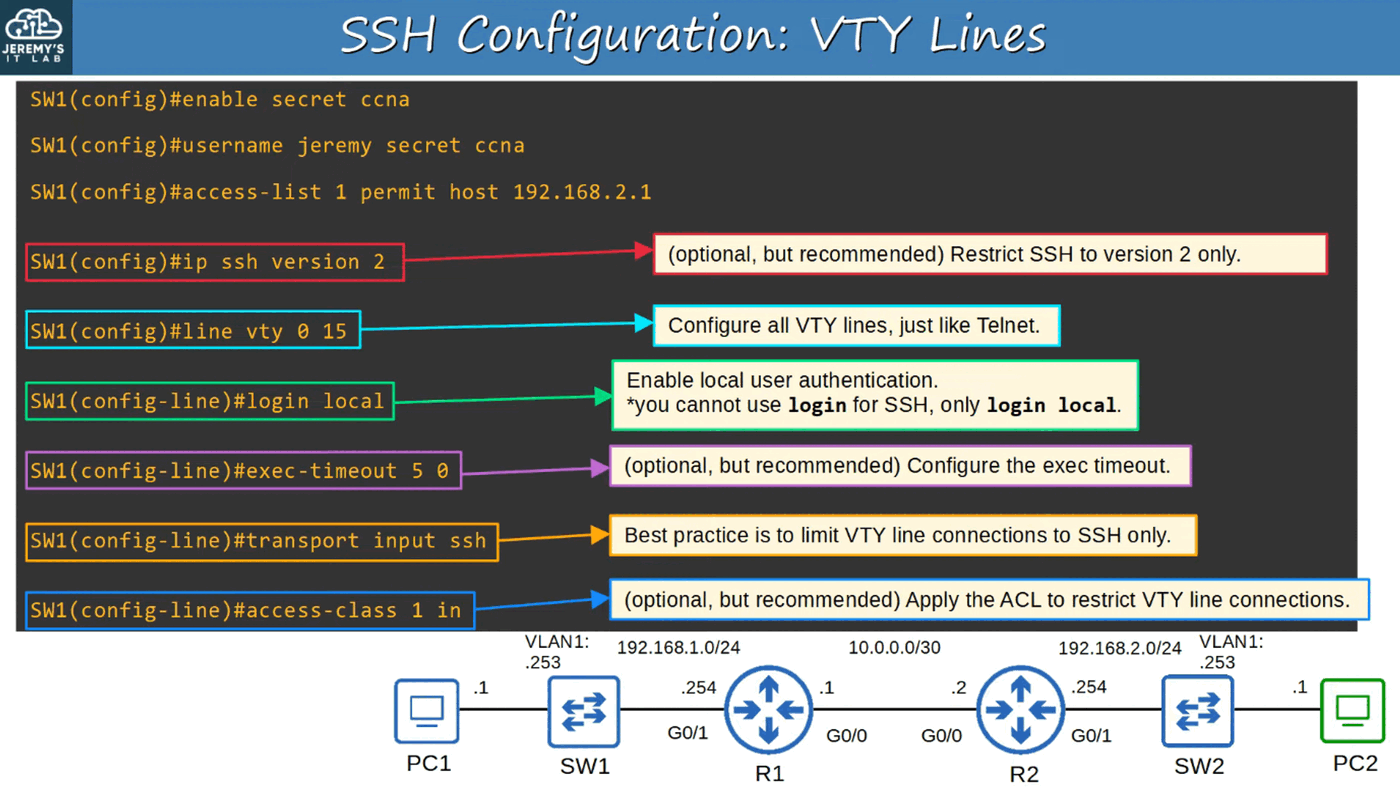
\includegraphics[keepaspectratio,alt={image}]{images/43-ssh/img-008.png}}
\end{figure}

\section{Summary About SSH
Configurations}\label{summary-about-ssh-configurations}

\begin{figure}
\centering
\pandocbounded{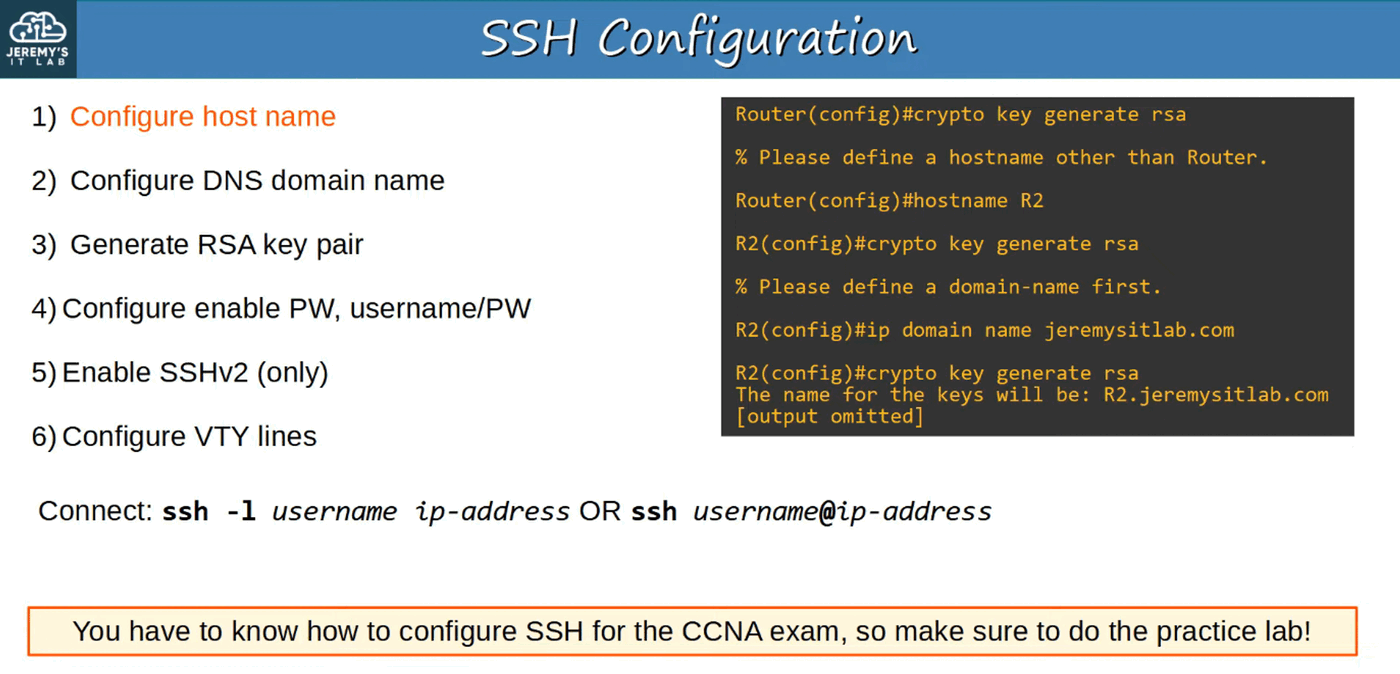
\includegraphics[keepaspectratio,alt={image}]{images/43-ssh/img-009.png}}
\end{figure}

\begin{figure}
\centering
\pandocbounded{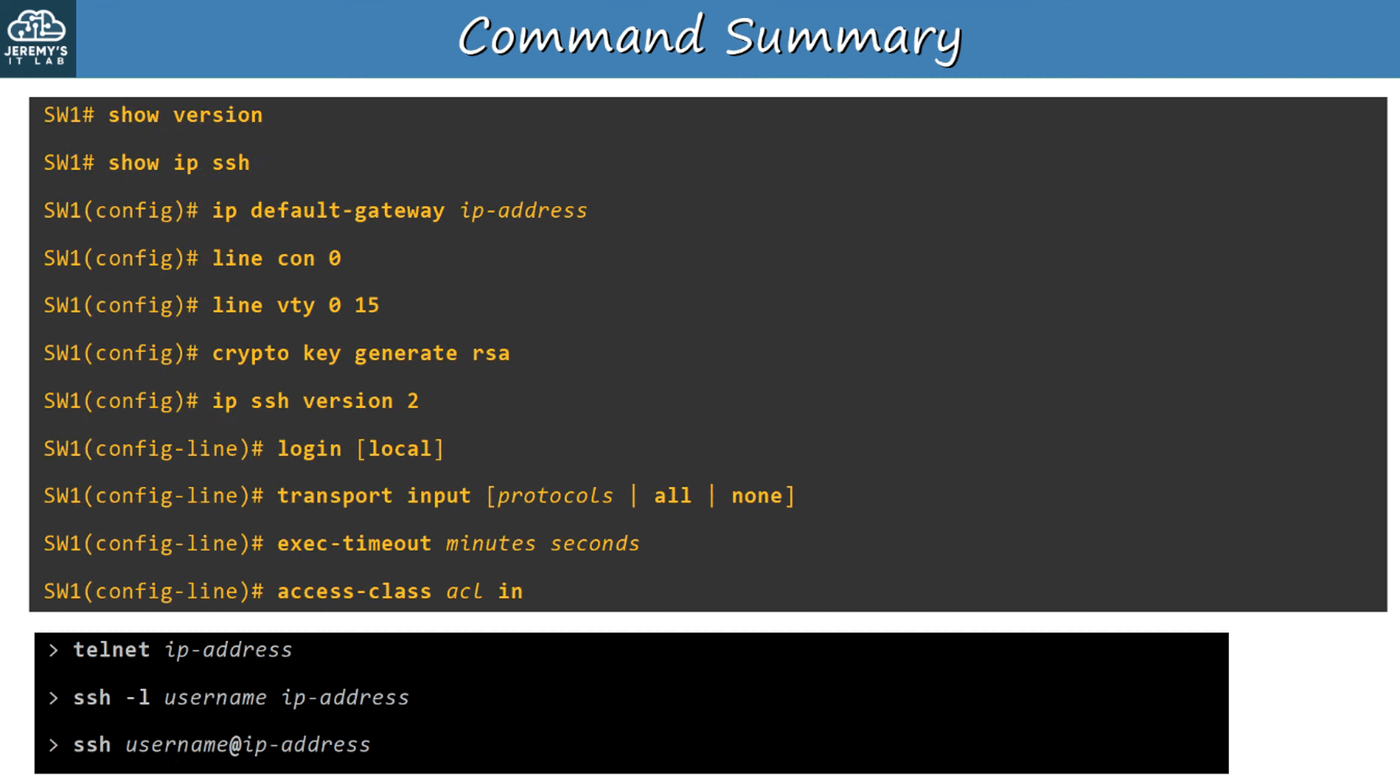
\includegraphics[keepaspectratio,alt={image}]{images/43-ssh/img-010.png}}
\end{figure}
